\chapter{Planificación y evaluación de costes}
\label{chap:planificacion}


Todo proyecto debería de disponer de una planificación inicial para establecer un guión a seguir, asegurando de esta manera el cumplimiento de los plazos, costes y calidad del producto final. A lo largo de este capítulo se detallará la planificación realizada para llevar a cabo el proyecto. 

En un primer punto se mostrarán los recursos que han participado en el proyecto y las tareas en las que se ha divido. Con estos datos definidos podemos establecer la planificación determinando de esta manera su línea base\footnote{Es una foto fija de la planificación a efectos de comparación.}.

Al finalizar el proyecto se compararán los resultados estimados con los reales, con la finalidad de ver las  desviaciones obtenidas.

En la última sección de este capítulo se realizará un análisis de riesgos, para intentar controlar algunos puntos que creemos que son críticos.

\section{Recursos y actividades}

Para la elaboración de cualquier proyecto primero deberemos conocer los recursos que tenemos y su disponibilidad, de la misma manera deberemos dividir nuestro proyecto en tareas más pequeñas con el fin de poder gestionarlas mejor.

Para este proyecto se contaron con los recursos que se mostrarán en la Tabla \ref{tab:recurso} y las siguientes tareas\footnote{Las tareas con horas son condicionados en esfuerzo y en días son condicionadas en duración.}:


\begin{enumerate}
    \item \textbf{Iteración 0: Búsqueda de información sobre el dominio}
    
    
    \begin{itemize}
        \item \textbf{Recopilación de información (80 horas)}: Búsqueda de información relacionada con el dominio de autenticación usando dispositivos móviles y técnicas de \textit{IA}.
        
        \item \textbf{Elaborar los requisitos (5 días)} : Se decidió elaborar una lista de requisitos que debería cumplir la aplicación para su correcto funcionamiento.
        
        \item \textbf{Peer Review Requisitos (2 días )} : La lista de requisitos elaborada se ha sometido a la revisión por parte de los directores.
    
        \item \textbf{Elaborar arquitectura - diseño de alto nivel (40 horas)} : Se describen los componentes principales del sistema y el modo en que interactúan entre sí. Elección de tecnologías, modelo arquitectónico junto con sus componentes.
    
        \item \textbf{Detalle de componentes (80 horas)}:  Último paso en la descomposición del diseño, en el que se llega a las unidades de programación (las clases de implementación) detallando los componentes identificados en el diseño de alto nivel. Diagrama final de clases, diagramas de secuencia, etc.
    \end{itemize}
    
    \item \textbf{Iteración 1:  Sistema de captura de información}
    \begin{itemize}
        \item \textbf{Elaborar pruebas (40 horas)}: Se elaboraran las pruebas para validar el correcto funcionamiento de la aplicación.
        
        \item \textbf{Implementación (240 horas)}: Se realizará el código de la aplicación siguiendo los parámetros establecidos.
        
        \item \textbf{Ejecutar pruebas (2 días)}: Se ejecutarán las pruebas preparadas en la tarea anterior.
    \end{itemize}
    
    \item \textbf{Iteración 2:  Sistema para el almacenamiento de la información}
    \begin{itemize}
        \item \textbf{Elaborar pruebas (40 horas)}: Se elaboraran las pruebas para validar el correcto funcionamiento del servidor.
        
        \item \textbf{Implementación (120 horas)}: Se realizará el código del servidor siguiendo los parámetros establecidos.
        
        \item \textbf{Ejecutar pruebas (2 días)}: Se ejecutarán las pruebas preparadas en la tarea anterior.
    \end{itemize}
    
    \item \textbf{Iteración 3: Comunicar la aplicación con servidor}
    \begin{itemize}
        
        \item \textbf{Desplegar Servidor (1 día)}: Es esta tarea se usará un servidor para que nuestro sistema sea accesible en cualquier momento.
        
        \item \textbf{Comunicar servidor y aplicación (5 días)}: Se establecerán las conexiones y configuraciones necesarias, para que ambos sistemas se comuniquen.
        
        \item \textbf{Securizar conexiones (3 días) }: Se creará un certificado digital y se configurará el servidor y la aplicación para que cifren las conexiones. 
        
    \end{itemize}
    
    \item \textbf{Iteración 4: Implementación de la Inteligencia Artificial}
    \begin{itemize}
    
    
        \item \textbf{Obtener datos (30 días)}: Se buscarán voluntarias para probar el sistema creado y conseguir los eventos necesarios para su posterior análisis.
        
        \item \textbf{Analizar características (240 horas)} : Analizar los datos recogidos y extraer sus características para el entrenamiento.
        
        \item \textbf{Implementar técnicas de Inteligencia Artificial (112 horas)}: Estudiar los distintos algoritmos para implementar la inteligencia artificial y programarla.
    
    \end{itemize}
    
    \item \textbf{Iteración 5:  Implementación online de los algoritmos}
        \begin{itemize}
            \item \textbf{Implementación online (32 horas)}: Crear un servidor que habilite el acceso al algoritmo implementado y responda con la predicción.
        \end{itemize}

    \item \textbf{Documentación del proyecto}: Elaborar la memoria del proyecto y otra documentación sobre instalación y configuración del proyecto. Esta tarea de documentación no tiene una duración establecida, ya que se desarrollará a lo largo de todo el proyecto.
    
\end{enumerate}


\begin{table}[!h]
    \centering
    \begin{tabular}{l l}
        \toprule
         Recurso & Coste~\cite{boe} \\
        \midrule
         Programador    &  10 \euro / hora \\
         Analista       &  12 \euro / hora \\
         Diseñador      &  10 \euro / hora \\
         Director       & 17 \euro / hora \\
         Servidor       & 0.013 \euro /hora \\
         Servidores para entrenamiento IA   &  0.70 \euro /hora \\
         Samsung Tab S4 & 600 \euro   \\
         Ordenador      & 650 \euro \\
        \bottomrule
    \end{tabular}
    \caption[Recursos del proyecto]{Recursos del proyecto~\protect\footnotemark}
    \label{tab:recurso}
\end{table}

\footnotetext{Los roles de programador, analista y diseñador han sido realizados por la misma persona.}

\section{Planificación Inicial}

La planificación inicial estima como deberá de ejecutarse todo el proyecto, las relaciones entre las tareas y los recursos asignados a estas. En la Figura~\ref{fig:tareas} se pueden ver las tareas planificadas con el coste, tiempo y dependencias de nuestro proyecto y la Figura~\ref{fig:gantt} muestra el \textit{Diagrama de Gantt}\footnote{Mapa donde se muestran las tareas relacionadas a lo largo del tiempo}.


\begin{landscape}

    \begin{figure}
            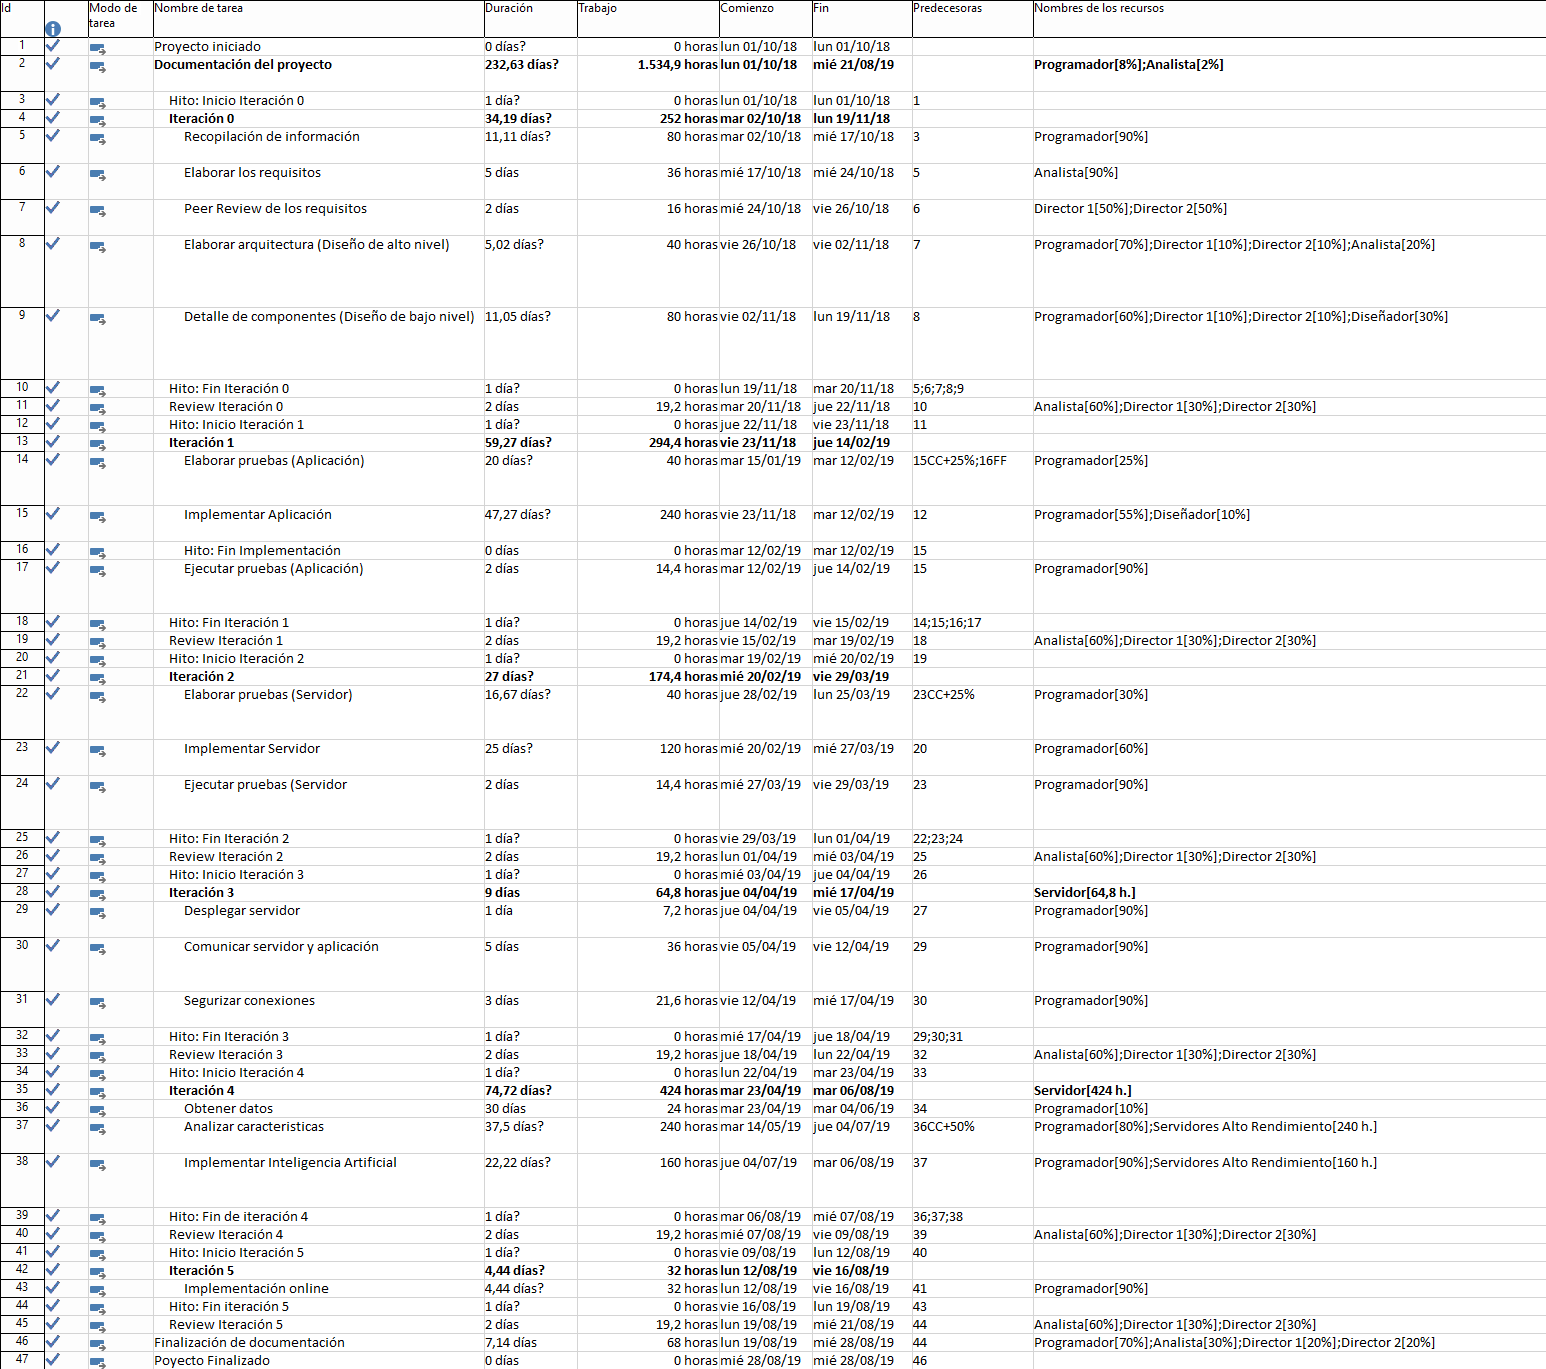
\includegraphics[width=\linewidth, height=0.9\textheight]{imaxes/project/tareas.png}
        \centering
        \caption{Lista de tareas planificadas}
        \label{fig:tareas}
    \end{figure}

    \begin{figure}
        \centering
        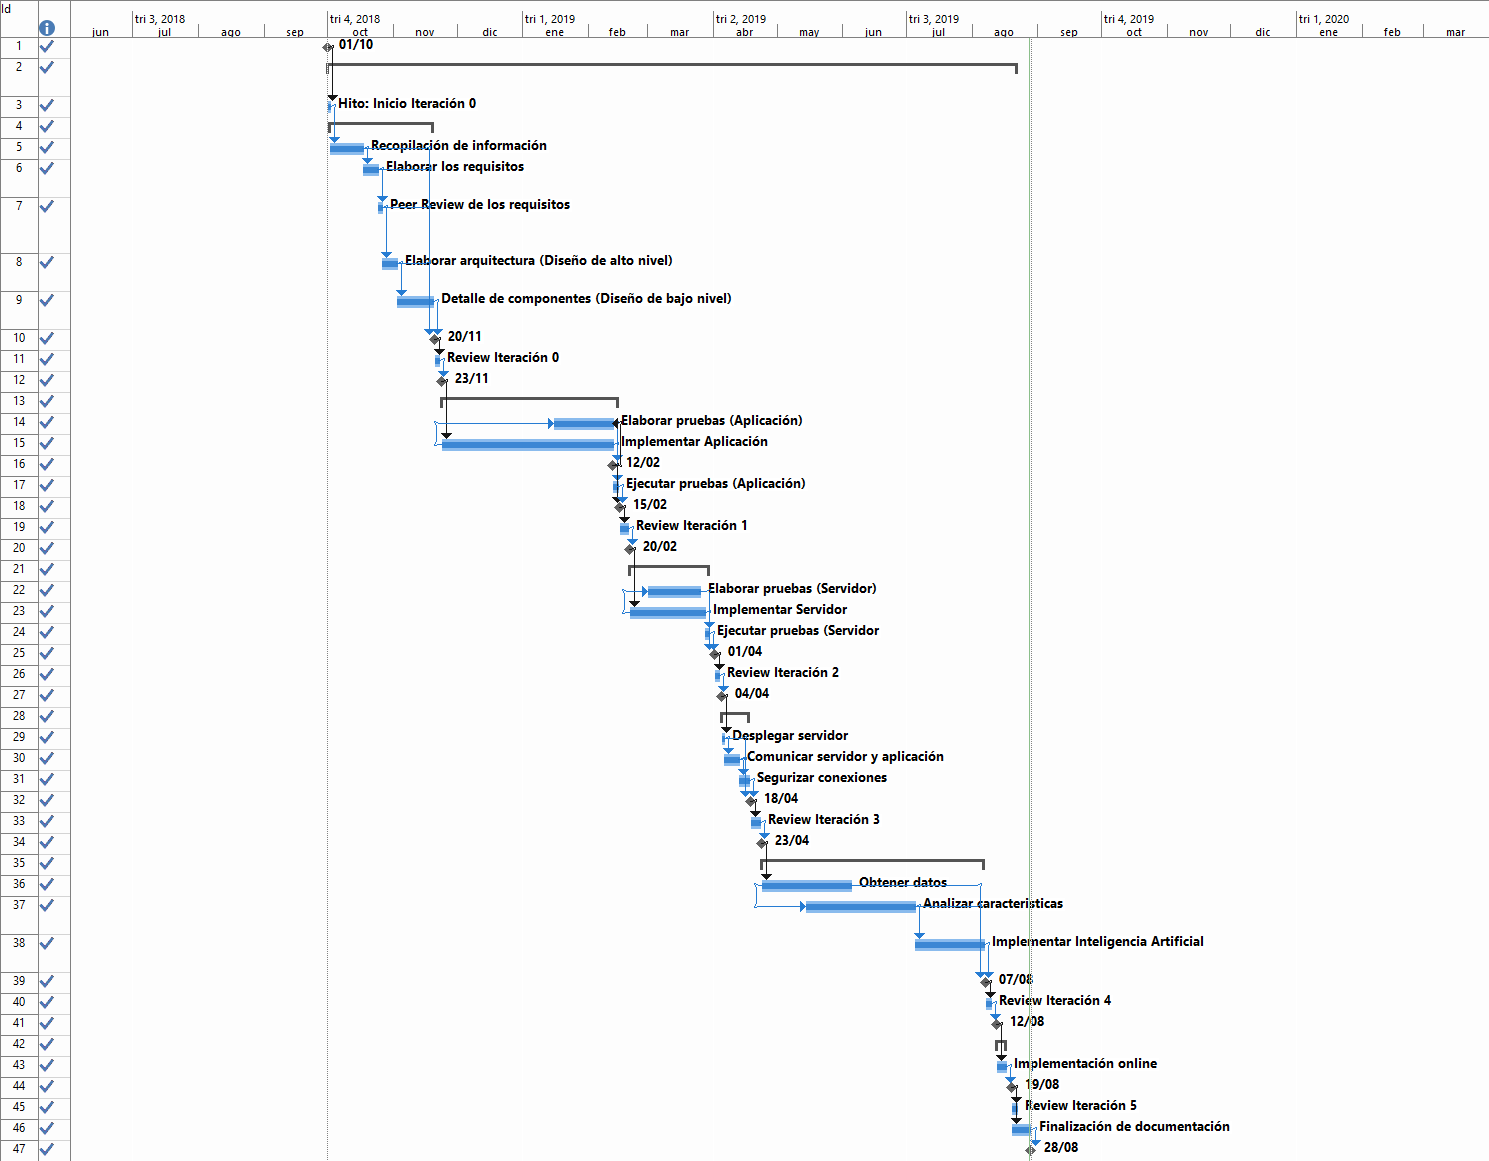
\includegraphics[width=\linewidth, height=0.9\textheight]{imaxes/project/gantt.png}
        \caption{Diagrama de Gantt}
        \label{fig:gantt}
    \end{figure}
\end{landscape}


\section{Seguimiento del proyecto}

En esta sección se detalla el seguimiento realizado sobre el proyecto a su finalización, ya que, durante el transcurso del proyecto se produjeron algunos retrasos.

Durante las fechas comprendidas entre el 23/12/2018 y el 6/1/2019, el \textit{Programador} se ausentó por motivos personales, y el proyecto tuvo que paralizarse durante esos días.
Una vez finalizado el proyecto se analizaron las desviaciones con respecto a la planificación estimada~[Tabla~\ref{tab:project_cost}]. La comparación de los datos muestran que debido a la ausencia \textit{Programador} durante esos días el proyecto sufriera ese mismo retraso en días.

\begin{table}[!h]
    \centering
    \begin{tabular}{ l r r }
        \toprule
        {} & Estimación & Real \\
        \midrule
        \textbf{Fecha Inicio}   & 1/10/2018         & 1/10/2019\\
        \textbf{Fecha Fin}      & 14/08/2019        & 28/8/2019 \\
        \textbf{Trabajo}        & 1.378,17~horas    & 1378.17~horas \\
        \textbf{Duración}       & 227,77~días       & 237,77~días \\
        \textbf{Costo}          & 18.607,93~\euro   & 18.607,93~\euro \\
        \textbf{Variación}      & {}                & 10 días \\ 
        \bottomrule
    \end{tabular}
    \caption[Costes y tiempos del proyecto]{Costes y tiempos del proyecto~\protect\footnotemark}
    
    \label{tab:project_cost}
\end{table}
\footnotetext{Mirando la fila de fecha de fin se observa que hay 14 días de diferencia, pero estos son naturales y no laborables}


\section{Análisis de riesgos}
A la hora de planificar un proyecto hay que tener en cuenta los riesgos de este. Por muy bien planificado que se encuentre sino se tienen en cuenta los riesgos, la planificación puede verse totalmente desajustada.

A la hora de preparar un plan de riesgos se siguen ciertos pasos ya establecidos:
\begin{itemize}
    \item \textbf{Identificación}: Elaborar un lista de posibles riesgos.
    \item \textbf{Valoración}: Cuantificar los riesgos para conocer el impacto que tendrían.
    \item \textbf{Análisis}: Estudiar alternativas y crear planes de prevención y contención.
\end{itemize}

Para este proyecto se han identificado algunos riesgos [Tabla \ref{tab:riesgos}] que en caso de suceder podrían retrasar el proyecto. Para algunos de ellos se ha elaborado un plan de contingencia para para minimizar su impacto en caso de que ocurran~[Tabla~\ref{tab:contingencia}]. 

\begin{table}[h]
    \centering
    \begin{tabular}{p{0.15\linewidth} p{0.45\linewidth} l c}
        \toprule
        Nombre                    & Descripción & Prob. & Impacto\\
        \midrule
        Conocimiento del dominio &  El dominio del proyecto es prácticamente desconocido para el autor. & Alto & Medio \\ \\
        
        Análisis de los datos  & Buscar características que sean identificativas del usuarios.  & Alto & Alto \\ \\
        
        Técnicas de IA  & Buscar técnicas o métodos que obtengan resultados concluyentes. & Alto & Alto \\ \\
        
        Configuración del sistema &  La configuración de cada una de las partes puede llegar a ser bastante complicada en ciertos puntos y generar conflictos. & Media  &  Bajo \\ \\
        
        Caída de servidores & Los servidores pueden sufrir caídas y dejar sin servicio.  & Media  &  Bajo \\ \\
        
        \bottomrule
    \end{tabular}
    \caption{Tabla de riesgos}
    \label{tab:riesgos}
\end{table}


\begin{table}[h]
    \centering
    \begin{tabular}{ l p{0.6\linewidth}}
         \toprule
         Riesgos & Plan de Gestión \\
         \midrule
          Configuración del sistema &  Tener una copia de seguridad actualizada con toda la configuración y servicios necesarios, para poder volver a una configuración estable \\
          Caída de servidores & Se ha decidido utilizar un servicio en la nube con alta disponibilidad para evitar que el riesgo ocurra.\\
         \bottomrule
    \end{tabular}
    \caption{Plan de gestión de riesgos}
    \label{tab:contingencia}
\end{table}

